\documentclass[a4j,11pt]{jarticle}
%\usepackage[dviout]{graphicx}
\usepackage[dvipdfmx]{graphicx}
\usepackage{amsmath}
\usepackage{amssymb}
\usepackage{ascmac}
%\usepackage{epsbox}
\usepackage{float}
\usepackage{here}
\usepackage{lscape}
\usepackage{latexsym}
\usepackage{pifont}
\usepackage{wrapfig}
\usepackage{type1cm}
\usepackage{algorithm}
\usepackage{algorithmic}
\usepackage{txfonts}
\usepackage{bm}
\usepackage{comment}
\usepackage{url}
%\usepackage{natbib}
%\usepackage[square]{natbib}

\usepackage{listings}
%\usepackage{plistings}

%\setlength{\voffset}{-25.4mm}
\setlength{\topmargin}{-17.5mm}   %トップとヘッダの間隔
%\setlength{\headheight}{20mm}   %ヘッダの高さ
%\setlength{\headsep}{0mm}   %ヘッダとテキストの間隔
\setlength{\textwidth}{45zw}   %テキストの幅
\setlength{\hoffset}{-10mm}
\setlength{\textheight}{45\baselineskip}   %テキストの高さ
%\addtolength{\textheight}{\topskip}
%\setlength{\footskip}{0mm}
%\setlength{\oddsidemargin}{21.5mm}   %サイドとテキストの間隔(奇数ページ)
%\setlength{\evensidemargin}{21.5mm}   %サイドとテキストの間隔(偶数ページ)
\pagestyle{empty}   %ページ番号なし
\newcommand{\g}[1]{\boldsymbol{#1}}
\newcommand{\lw}[1]{\smash{\lower2.0ex\hbox{#1}}}
\renewcommand{\baselinestretch}{1.0}

\makeatletter
\def\theequation{\arabic{equation}}   %数式番号を(章.式)形式
\@addtoreset{equation}{section}
%\def\thefigure{\thesection.\arabic{figure}}   %図番号を(章.図)形式
%\@addtoreset{figure}{section}
%\def\thetable{\thesection.\arabic{table}}   %表番号を(章.表)形式
%\@addtoreset{table}{section}
\def\tr{\mathop{\operator@font tr}\nolimits}
\def\grad{\mathop{\operator@font grad}\nolimits}
\def\St{\mathop{\operator@font St}\nolimits}
\def\Hess{\mathop{\operator@font Hess}\nolimits}
\def\D{\mathop{\operator@font D}\nolimits}
\def\sym{\mathop{\operator@font sym}\nolimits}
\def\s.t.{\mathop{\operator@font s.t.}\nolimits}
\def\diag{\mathop{\operator@font diag}\nolimits}
\def\section{\@startsection{section}{1}{\z@}
   {0.8\Cvs \@plus.5\Cdp \@minus.2\Cdp}
   {0.2\Cvs \@plus.3\Cdp}
   {\normalfont \Large \bfseries}}
\makeatother
\makeatletter
\def\subsection{\@startsection{subsection}{1}{\z@}
   {0.8\Cvs \@plus.5\Cdp \@minus.2\Cdp}
   {0.2\Cvs \@plus.3\Cdp}
   {\normalfont \normalsize \bfseries}}
\makeatother
\makeatletter
\newcommand{\figcaption}[1]{\def\@captype{figure}\caption{#1}}
\newcommand{\tblcaption}[1]{\def\@captype{table}\caption{#1}}
\makeatother

\begin{document}
%\bibliographystyle{jecon}
%\bibliographystyle{apalike} %いらない

\begin{center}
{\Large \textbf{混合 Projected Normal 分布によるクラスタリングの性能評価}}
\end{center}
\begin{flushright}
小坪 琢人(塩濱 敬之准教授)
\end{flushright}
\vspace{-3zh}

%%%%%%%%%%%%% これ以下, 本文 %%%%%%%%%%%5%%
%%%%%%%%%%%%%  section1  はじめに %%%%%%%%%%%%%%%

\section{はじめに}

\begin{wrapfigure}[10]{r}[5mm]{70mm}
\vspace{-0.6cm}
\centering
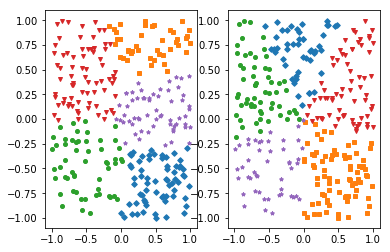
\includegraphics[keepaspectratio,width=70mm]{data/kmeans+skmeans.png}
\vspace{-1cm}
\caption{k-meansによるクラスタリング(左), skmeansによるクラスタリング(右)}
\label{kmeans}
\end{wrapfigure}

$k$-means法は, 各データと各クラスタの中心のユークリッド距離を最小化することで, 各データをクラスタリングする. しかしデータが単位超球面上に配置されている場合, 同一方向のデータを別々のクラスタに分割することがある. そこで spherical $k$-means (skmeans) 法では各データを正規化し, 各データを単位方向ベクトルとする. このようなベクトルを指向性データ(directional data)と呼ぶ. データの単位方向ベクトルと各クラスタにおける重心ベクトルとのコサイン非類似度を最小化することで, 各データをクラスタリングする. 図\ref{kmeans}に$k$-means法と skmeans法によるクラスタリング分析例を示す. 

上記のノンパラメトリックな手法に対し, パラメトリックな超球面上のクラスタリング手法として, S. Gopal and Y. Yang(2014) による Von Mises Fisher 分布の混合分布を用いた手法がある. 混合ガウスモデルと同様に, データを複数の Von Mises Fisher 分布から再現できると仮定して, 各分布のパラメータをマルコフ連鎖モンテカルロ法(MCMC)により逐次計算する. MCMCを用いることで求める分布のパラメータの平均値, 標準偏差を求めることができる. 本研究では方向データの分布として知られる, Projected Normal 分布の混合分布によるクラスタリングの性能評価を行う. Projected Normal 分布はパラメータによって, 単峰性・二峰性の形状を取ることができるので, 多峰性のデータをクラスタリングする際に混合 Von Mises Fisher 分布によるクラスタリングとどのような差異が現れるか比較する.

%%%%%%%%%%%%%%%%%%%%%%%%%%%%%%%%%%%%%%%%%%%%%%%%%%%%%%%%%%%%%%%%%%%%%%%%%%%%%%%%%%%%%%%%%%%%%%%%%%%%%%%%%%%%%%%
%%%%%%%%%%%%%%%%%%%%%%%% senction2 混合分布 %%%%%%%%%%%%%%%%%%%%%

\section{混合 Projected Normal 分布}
\vspace{-0.5zh}
\subsection{Projected Normal 分布}

Projected 分布は平面または空間上の放射状の射影によって得られる. より一般的には, 多変量正規ベクトルをノルムで割ることで, 単位超球面上への射影分布が得られる. 多変量正規ベクトル($k$次元)を$X$として, $k \geq 2$ の場合には, 単位超球面上への単位ベクトル $U$ は $U = X/||X||$ で表される. このとき$U$は$k$次元の General Projected Normal 分布に従い, $U \sim \mathcal{PN}_k(\bm \mu,\Sigma)$と表せる. General Projected Normal 分布は, パラメータ$\bm \mu, \Sigma$をもち, Presnell. B(1998) らによる, $\Sigma = \mathcal{I}$と定義されていたProjected Normal 分布を一般化したものである. $\mathcal{PN}_k(\bm \mu,\mathcal{I})$は平均方向$\bm \mu$に対して, 単峰性かつ対称の分布となるが, $\mathcal{PN}_k(\bm \mu,\Sigma)$では対称分布もしくは二峰性分布となる.

Wang and Gelfand (2013) によると,$\Sigma \neq I$のもとで$\mathcal{PN}_2(\bm \mu,\Sigma$)のとき, 円形データの場合, 単位円上の方向を表す$U = (\cos\Theta, \sin\Theta)^T$における$\theta$の確率密度は以下で表す.

\vspace{-0.5zh}
\begin{eqnarray*}
\label{PNC}
p(\theta; \bm \mu, \Sigma) = \frac{1}{2\pi A(\theta)}|\Sigma|^{-\frac{1}{2}}
\exp(C)\left\{1 + \frac{B(\theta)}{\sqrt{A(\theta)}} \frac{\Phi \left(\frac{B(\theta)}{\sqrt{A(\theta)}}\right)}{\phi \left(\frac{B(\theta)}{\sqrt{A(\theta)}}\right)}\right\} I_{[0,2\pi)}(\theta)
\end{eqnarray*}

\noindent
$\bm u^T = (\cos\theta,\sin\theta), A(\theta) = \bm u^T\Sigma^{-1}\bm u, B(\theta) = \bm u^T \Sigma^{-1} \bm \mu, C = -\frac{1}{2} \bm \mu^T \Sigma^{-1} \bm \mu$であり, $I_{[0,2\pi)} (\cdot)$は指示関数, $\Phi(\cdot),\phi(\cdot)$ は標準正規分布の確率密度関数と累積密度関数である.

\newpage
\vspace{-0.5zh}
\subsection{混合 Projected Normal 分布}

単位円上における, $m$個のユニットからなる Projected Normal 分布の混合分布は以下のように定式化できる. 

\vspace{-1zh}
\begin{eqnarray*}
p(\theta;\bm w,\bm \mu, \Sigma) = \sum^m_{j=1} w_j \mathcal{PN}_2(\theta;\bm \mu_j, \Sigma_j) 
\end{eqnarray*}

\noindent
ただし, $w_j$は各ユニットの重みであり, $0 < w_j < 1$, $\sum^m_{j=1} w_j = 1$を満たす.

\noindent
ここで両辺の対数を取ると, 

\vspace{-1zh}
\begin{eqnarray*}
\log p(\theta; w_j, \bm \mu, \Sigma) &=& \sum^m_{j=1} \{\log w_j + \log \mathcal{PN}_2(\theta; \mu_j, \Sigma_j)\} \\
&=& \sum^m_{j=1} \left[ \log w_j - \log 2\pi - \log A - \frac{1}{2} \log |\Sigma| + C + \log \left\{1 + \frac{B(\theta)}{\sqrt{A(\theta)}} \frac{\Phi \left(\frac{B(\theta)}{\sqrt{A(\theta)}}\right)}{\phi \left(\frac{B(\theta)}{\sqrt{A(\theta)}}\right)}\right\} \right] \\
&\propto& \sum^m_{j=1} \left[ \log w_j - \log A - \frac{1}{2} \log |\Sigma| + C + \log \left\{1 + \frac{B(\theta)}{\sqrt{A(\theta)}} \frac{\Phi \left(\frac{B(\theta)}{\sqrt{A(\theta)}}\right)}{\phi \left(\frac{B(\theta)}{\sqrt{A(\theta)}}\right)}\right\} \right]  
\end{eqnarray*}

\vspace{-0.5zh}\noindent
最後の式変形では, 対数尤度を計算するときに, 定数項は尤度に影響を与えないので消去する.

%%%%%%%%%%%%%%%%%%%%%%%%%%%%%%%%%%%%%%%%%%%%%%%%%%%%%%%%%%%%%%%%%%%
%%%%%%%%%%%%%%%%%%%%%%%  sectio3 解析手法 %%%%%%%%%%%%%%%%%%%%%%%%

\section{解析手法}

\vspace{-0.5zh}
\subsection{マルコフ連鎖モンテカルロ法}

本研究ではMCMCアルゴリズムの一つである, ハミルトニアンモンテカルロ法(HMC)を用いて実験を行う.

%%%%%%%%%%%%%%%%%%%%%%%  HMC法について記述する %%%%%%%%%%%%%%%%%%%%%%%%%%%%%%%%%%%%

\vspace{-0.5zh}
\subsection{パラメータの推定手法}

Projected Normal 分布におけるパラメータは, $\bm \mu,\Sigma$ であるが, 識別可能性を保持するという制約を加えると, 共分散行列$\Sigma$は以下で定義される.
\vspace{-0.5zh}
\[
 \Sigma = \left(
    \begin{array}{cc}
      \tau^2 & \rho \tau \\
      \rho \tau & 1
    \end{array}
  \right)
\]

よって推定すべきパラメータは$\bm \mu, \tau, \rho, \bm w$となる. Wang and Gelfand (2013)の研究から, 各パラメータの事前分布を $\bm \mu \sim N(\bm 0, 10^5 \bm I_2)$, $\tau \sim \mathrm{half Cauchy}(0,5)$, $\rho \sim U(-1,1)$, $\bm w \sim Dirichlet(2,2, \cdots, 2)$ と設定する. ここで重みパラメータ$\bm w$は$m$次元の$Dirichlet$分布に従うものとする. 

%%%%%%%%%%%%%%%%%%%%%%%%%%%%%%%%%%%%%%%%%%%%%%%%%%%%%%%%%%%%%%%%%%%
%%%%%%%%%%%%%%%%%%%%%%%  sectio4 数値実験 %%%%%%%%%%%%%%%%%%%%%%%%

\section{データ解析}

人工的データを用いて, 混合 Projected Normal 分布によるクラスタリングの性能評価を行う.

\subsection{解析データ}


%%%%%%%%%%%%%%%%%%%%%%%%%%%%%%%%%%%%%%%%%%%%%%%%%%%%%%%%%%%%%%%%%%%%%%
%%%%%%%%%%%%%%%%%%%%%%%  section5 まとめ %%%%%%%%%%%%%%%%%%%%%%%%%%%%%

\section{まとめ}


%\newpage
\addcontentsline{toc}{section}{参考文献} %目次に参考文献を入れる

%必要になる
%\newpage
%\section{付録}

%参考文献を引用する際に必要なコマンド
\bibliographystyle{jplain}
\bibliography{bunken}

%%%%%%%%%%%%%%%%%%%%%%%%%%%%%%%%%%%%%%%%%%%%%%%%%%%%%%%%%%%%%%%%%%%
%%%%%%%%% 参考文献用 bibtexから呼び出すページ %%%%%%%%%%%%%%%%%%%%%%%%%%

\newpage

関係ないページです!

Presnell. B(1998) \cite{PML}

Wang and Gelfand (2013) \cite{PN1}

D. Hemandez(2017) \cite{GPN}

S. Gopal and Y. Yang(2014) \cite{Gopal}
\vspace{-0.3cm}
\begin{figure}[H]
\begin{center}
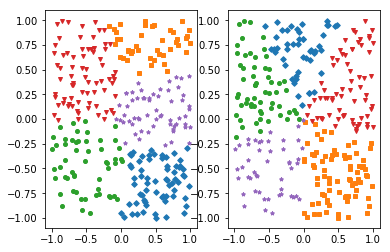
\includegraphics[clip,height= 35mm]{data/kmeans+skmeans.png}
\end{center}
 \vspace{-0.9cm}
\caption{k-meansによるクラスタリング(左), skmeansによるクラスタリング(右)}
\label{skmeans}
\end{figure}

\end{document}

%\begin{table}[H]
%\begin{center}
%\caption{条件付確率表(CPT)}   %キャプション
%\label{cpt}   %ラベル
%\begin{tabular}{|c||c|c|c|}   %{}で文字の揃え方を指定
%\hline
% & $Pa(X_{j})=x_{1}$ & \dots & $Pa(X_{j})=x_{m}$
%\\ \hline
%$X_j=y_1$ & $p(y_1|Pa(X_j)=x_1)$ & \dots & $p(y_1|Pa(X_j)=x_m)$
%\\ \hline
%$\vdots$ & $\vdots$ & $\ddots$ & $\vdots$
%\\ \hline
%$X_j=y_n$ & $ p(y_n|Pa(X_j)=x_1)$ & \dots & $p(y_n|Pa(X_j)=x_m)$
%\\ \hline
%\end{tabular}
%\end{center}
%\end{table}
